\subsection{Squares over Unordered Alphabets}

\begin{frame}
    \centering
    {\Large Optimal Square Detection  Over General Alphabets}
  
    \bigskip
    {\large SODA'23}\\
    \bigskip
    
\includegraphics{pictures/mindmap/squares.png}
  
    \bigskip
    Jonas Ellert, Paweł Gawrychowski
\end{frame}

\begin{frame}{Estimating the alphabet size}
    
    \begin{itemize}
    \item<1-> proceed in $\orderof{\lg\lg n}$ phases, with $\Delta_1 = \Theta(\sqrt{n})$ and $\Delta_{i + 1} = \sqrt{\Delta_i}$
    \vspace{.25\baselineskip}
    \item<2-> in phase $i$, try to detect square of length $\Omega(\Delta_i)$ and $\orderof{\Delta_{i + 1}} = \orderof{\Delta_i^2}$
    \end{itemize}
    
    \onslide<3->
    \vspace{\baselineskip}
    
    \begin{tikzpicture}
    
    
    \node (1-0) {$w = {}$};
    \foreach[evaluate=\i as \iminus using int(\i-1)] \i in {1,...,30} {
        \node[right=0 of 1-\iminus, minimum width=.9em] (1-\i) {\vphantom{a}};
        \node[below=.25em of 1-\i, minimum width=.9em] (1a-\i) {\vphantom{a}};
        \node[below=-.75em of 1-\i, minimum width=.9em] (1b-\i) {\vphantom{a}};
        \node[below=2em of 1-\i, minimum width=.9em] (2-\i) {\vphantom{a}};
    }
    
    
    \foreach[
    evaluate=\x as \firstx using int((\x-1)*6+1),
    evaluate=\x as \lastx using int(\x*6),
    ] \x in {1,...,5} {
    
    \node[fit=(1-\firstx)(1-\lastx), draw, inner sep=0pt] (1-x\x) {};
    \node at (1-x\x) {$B_{\x}$};
    }
    
    \foreach[
    evaluate=\x as \firstx using int((\x-1)*1+1),
    evaluate=\x as \lastx using int(\x*1),
    ] \x in {20,...,28} {
    
    \onslide<12->{\node[fit=(2-\firstx)(2-\lastx), draw, inner sep=0pt] (2-x\x) {};}
    }
    
    \foreach[
    evaluate=\x as \firstx using int((\x-1)*1+1),
    evaluate=\x as \lastx using int(\x*1),
    ] \x in {23,...,26} {
    
    \node<13->[fill=red, fit=(2-\firstx)(2-\lastx), draw, inner sep=0pt] (2-x\x) {};
    }
    
    
    
    \node<12->[left=0 of 2-20] {$\cdots$};
    \node<12->[right=0 of 2-28] {$\cdots$};
    
    \node<11->[fill=myorange, fit=(1b-21.north)(1b-28.south), draw, inner sep=0pt] (tj) {};
    \node<11-> at (tj.center) {$t_j$};
    
    \only<13->{
        \draw[thick, densely dotted] (tj.north west) to (tj.west |- 2-x23.south);
        \draw[thick, densely dotted] (tj.north east) to (tj.east |- 2-x23.south);
        \node<14->[below right=.5em and -2em of tj.east |- 2-x23.south] {$\implies \orderof{n \lg \sigma}$ time};
    }
    
    \node[below=3em of 2-1] {};
    
    
    \node[fit=(1a-1)(1a-6)] {\leftarrowfill};
    \node[fit=(1a-1)(1a-6)] (lenmark) {\rightarrowfill};
    \node[below=0 of lenmark.center] {$\Theta(\Delta_i^2)$};
    
    \node[above=3em of 1-1] {};
    
    % time, if $\sigma = \orderof{\sqrt[4]{\Delta_i}}$
    %{\orderof{\Delta_i^2 + \frac{(\Delta_i)^2 \cdot \lg \Delta_i \cdot \sigma}{\sqrt{\Delta_i}}} = \orderof{\Delta^2}}}
    
    \node<4->[above=-.2em of 1-x1.north east] (thebrace) {$\overbrace{\hspace{10.5em}}$};
    \node<5->[above=.25em of thebrace, inner sep=0] (thetime) {$\strut\orderof{\Delta_i^2 + \frac{(\Delta_i)^2 \cdot \lg \Delta_i \cdot \sigma}{\sqrt{\Delta_i}}}$ time};
    \node<6->[right=0 of thetime, inner sep=0] {, which is $\strut\orderof{\Delta_i^2}$ if $\sigma = \orderof{\sqrt[4]{\Delta_i}}$};
    \node<4->[below=-.2em of 1-x2.south east] {$\underbrace{\hspace{10.5em}}$};
    
    
    
    
    \end{tikzpicture}
    
    \vspace{-1.5\baselineskip}
    
    \begin{itemize}
    \item<7-> single phase takes $\orderof{n}$ time
    \vspace{.25\baselineskip}
    \item<8-> if $\sigma = \Omega(\sqrt[4]{\Delta_i})$, then $\orderof{\Delta_i^2 \lg (\Delta_i^2)} = \orderof{\Delta_i^2 \lg \sigma}$\\[.25\baselineskip]
    \onslide<9->$\implies$ run \textcolor{red}{\bfseries Main+Lorentz'84} on each block pair, finish in $\orderof{n \lg \sigma}$ time\\
    \onslide<10->$\implies$ total time $\orderof{n (\lg \sigma + \lg\lg n)}$ without knowing $\sigma$
    \end{itemize}
    
    
\end{frame}

\begin{frame}{Lowerbound on square detection}
    Player vs Adversary: aims at giving as little information as possible\\
    \begin{itemize}
        \item Keep track of the comparisons asked through a conflict graph.
        \item Divide the string in blocks of $\sigma/4$. 
        \item Separate the blocks by character of \ntheme{the Prouet-Thue-Morse square-free sequence}. $\implies$ square-free iff all blocks are square free.  
        \item \btheme{Coloring rule}: If a node/position reaches degree $\sigma/4$, we color it by \ntheme{avoiding} the color of \ntheme{the neighbours} + the colors of \ntheme{the same block}.
    \end{itemize}
    
    \begin{center}
        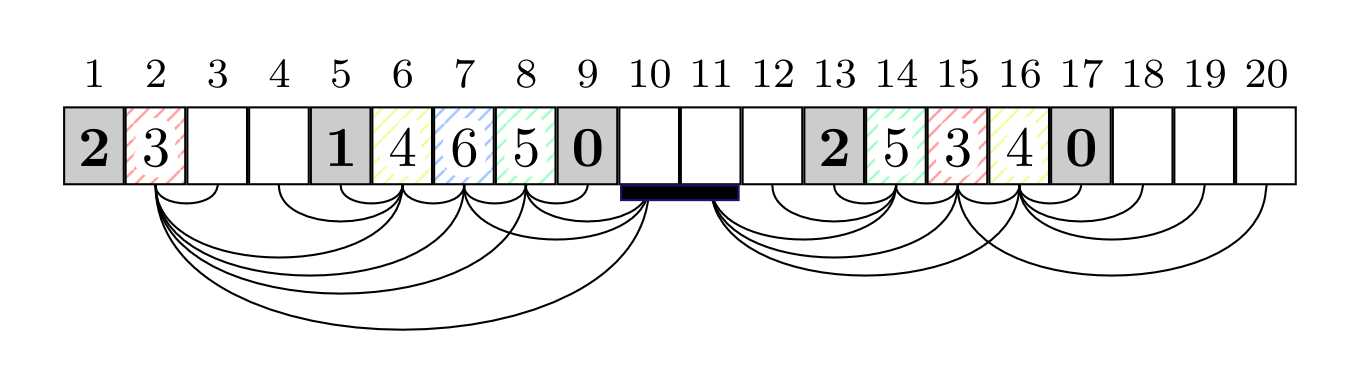
\includegraphics[width=0.5\textwidth]{pictures/squares_conflict.png}
    \end{center}

    Analysis of the conflict graph after the player terminates.
\end{frame}
